\chapter[Vision artificielle et humanités]{Vision artificielle et humanités : de la performance algorithmique à l'herméneutique des données}

\lettrine{L}{es} chercheurs et les institutions qui appliquent la vision artificielle aux corpus historiques se heurtent souvent à l'opacité technique de ces outils. Dès lors, la pertinence de ces technologies pour les humanités numériques ne se mesure pas à leur seule performance algorithmique, mais à la rigueur méthodologique avec laquelle elles s'articulent aux exigences d'une discipline et d'un programme de recherche spécifiques.

\section[La prise en main par les chercheurs]{La prise en main par les chercheurs : une dépendance technique et une divergence d'objectifs}

Le domaine des humanités et de l'analyse de documents n'utilise qu'une petite fraction des avancées du monde de la vision artificielle. La recherche et l'industrie informatique se concentrent aujourd'hui principalement sur d'autres problématiques comme la segmentation vidéo en temps réel ou la création de modèles génératifs multimodaux. De son côté, la vision patrimoniale se focalise sur une typologie de besoins bien précise : la classification, l'analyse de mise en page (layout analysis), la détection d'objets et, plus récemment la segmentation.

Ici sans prendre en compte les tầches d'\gls{ocr} et d'\gls{htr}, la vision artificielle appliquée aux corpus patrimoniaux s'articule autour de quatre tâches fondamentales dont la complexité et les coûts d'annotation varient sensiblement. 

\subsection{Les tâches la vision à visée patrimoniale}

\subsubsection{La classification globale} Elle vise à attribuer une étiquette unique à une image complète. Elle est adaptée à des tâches de tri relativement grossières qui, dans notre cadre, permettent le tri automatisé de grandes masses documentaires (distinction entre manuscrit et imprimé, identification du support, attribution du style d'une écriture). Son principale avantage vient d'un système d'annotation reposant sur une étiquette unique par image, et donc en utilisant également une ontologie simple.

\subsubsection{La détection d'objet et l'analyse de mise en page}
    
\begin{description}
    
    \item \textbf{La détection d'objets :} Reposant sur la délimitation par boîtes englobantes (\textit{bounding boxes}), elle permet de localiser et de catégoriser des entités visuelles discrètes au sein de la page. C'est l'outil privilégié des historiens de l'art et des codicologues pour repérer rapidement des lettrines, des sceaux, des filigranes ou des motifs iconographiques récurrents. Dans le projet AIKON, deux modèles de détection d'objets sont utilisés, un modèle de détection de diagramme et un modèle de détection d'illustration. Durant notre stage, l'une des stratégies que nous avons adoptées a été de rendre nos classes \og asémantiques\fg, c'est-à-dire de regrouper des éléments différents (illustrations ou diagrammes par exemple) sous une même bannière en dépit du sens dans le document pour privilégier une méthode d'annotation économique en temps et en moyens comme le montre l'image~\ref{fig:détection}. Bien plus coûteux que l'annotation d'une classification globale, le coût et la complexité de l'annotation pour l'analyse de mise en page dépendent des documents étudiés\footnote{Voir les grilles tarifaires moyennes des prestataires de labellisation de données (\textit{Data Annotation Pricing Guides}, 2025-2026 par DataVLab, Mindkosh AI et AI Superior) : le coût moyen d'une \textit{bounding box} varie entre 0,03 \$ et 0,08 \$ par objet, contre 0,50 \$ à 3,00 \$ par image pour une segmentation au pixel, traduisant un rapport de coût de 1 à 10 selon la complexité visuelle du document.}. 
    
    \item \textbf{L'analyse de mise en page (\textit{layout analysis}) :} C'est une sous-catégorie de la détection d'objets et une étape préalable indispensable à la lecture automatisée. Elle consiste à décomposer l'espace de la page pour en extraire la structure architecturale. Il s'agit d'isoler les blocs de texte principal, les gloses marginales, les colonnes, les en-têtes et les zones non textuelles afin de préserver l'ordre de lecture originel du document. Contrairement à la détection d'objets simple, les annotations sont donc divisées selon un sens de la mise en page et de la hiérarchie entre les éléments comme le montre l'image~\ref{fig:segmentation}. C'est l'une des formes d'annotations les plus coûteuses et les plus difficiles à mettre en œuvre, notamment à cause de la hiérarchie interclasse et de la relation entre les objets. La presse concentre la majorité des efforts car c'est l'un des domaines où la mise en page est complexe et coûteuse à annoter\footnote{ Benjamin Charles Germain Lee, Jaime Mears, Eileen Jakeway, Meghan Ferriter, Chris Adams, Nathan Yarasavage, Deborah Thomas, Kate Zwaard, Daniel S. Weld, \og The Newspaper Navigator Dataset: Extracting And Analyzing Visual Content from 16 Million Historic Newspaper Pages in Chronicling America\fg, publié sur ArXiv, 2020, URL : \href{https://arxiv.org/abs/2005.01583}{https://arxiv.org/abs/2005.01583}}. 
    
\end{description}
    
    %Bounding boxes: $0.02-$0.10 per object
    %Polygon annotations: $0.04-$0.15 per object
    %Semantic segmentation: $0.10-$3.00 per mask
    %3D point cloud labeling: $0.50-$5.00 per frame

\begin{figure}[htbp]
        \centering
        \begin{subfigure}{0.48\textwidth}
            \centering
            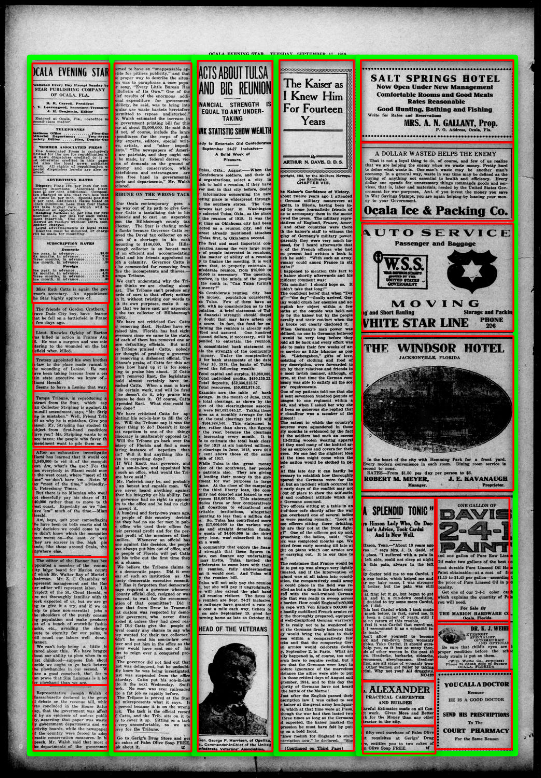
\includegraphics[scale=0.4]{img/segmentation.png}
            \caption{\textbf{Analyse de mise en page :} Exemple d'analyse simple de la mise en page d'une page de presse avec en vert les colonnes, et en rouge la segmentation des articles.}
            \label{fig:segmentation}
        \end{subfigure}
        \hfill
        \begin{subfigure}{0.48\textwidth}
            \centering
            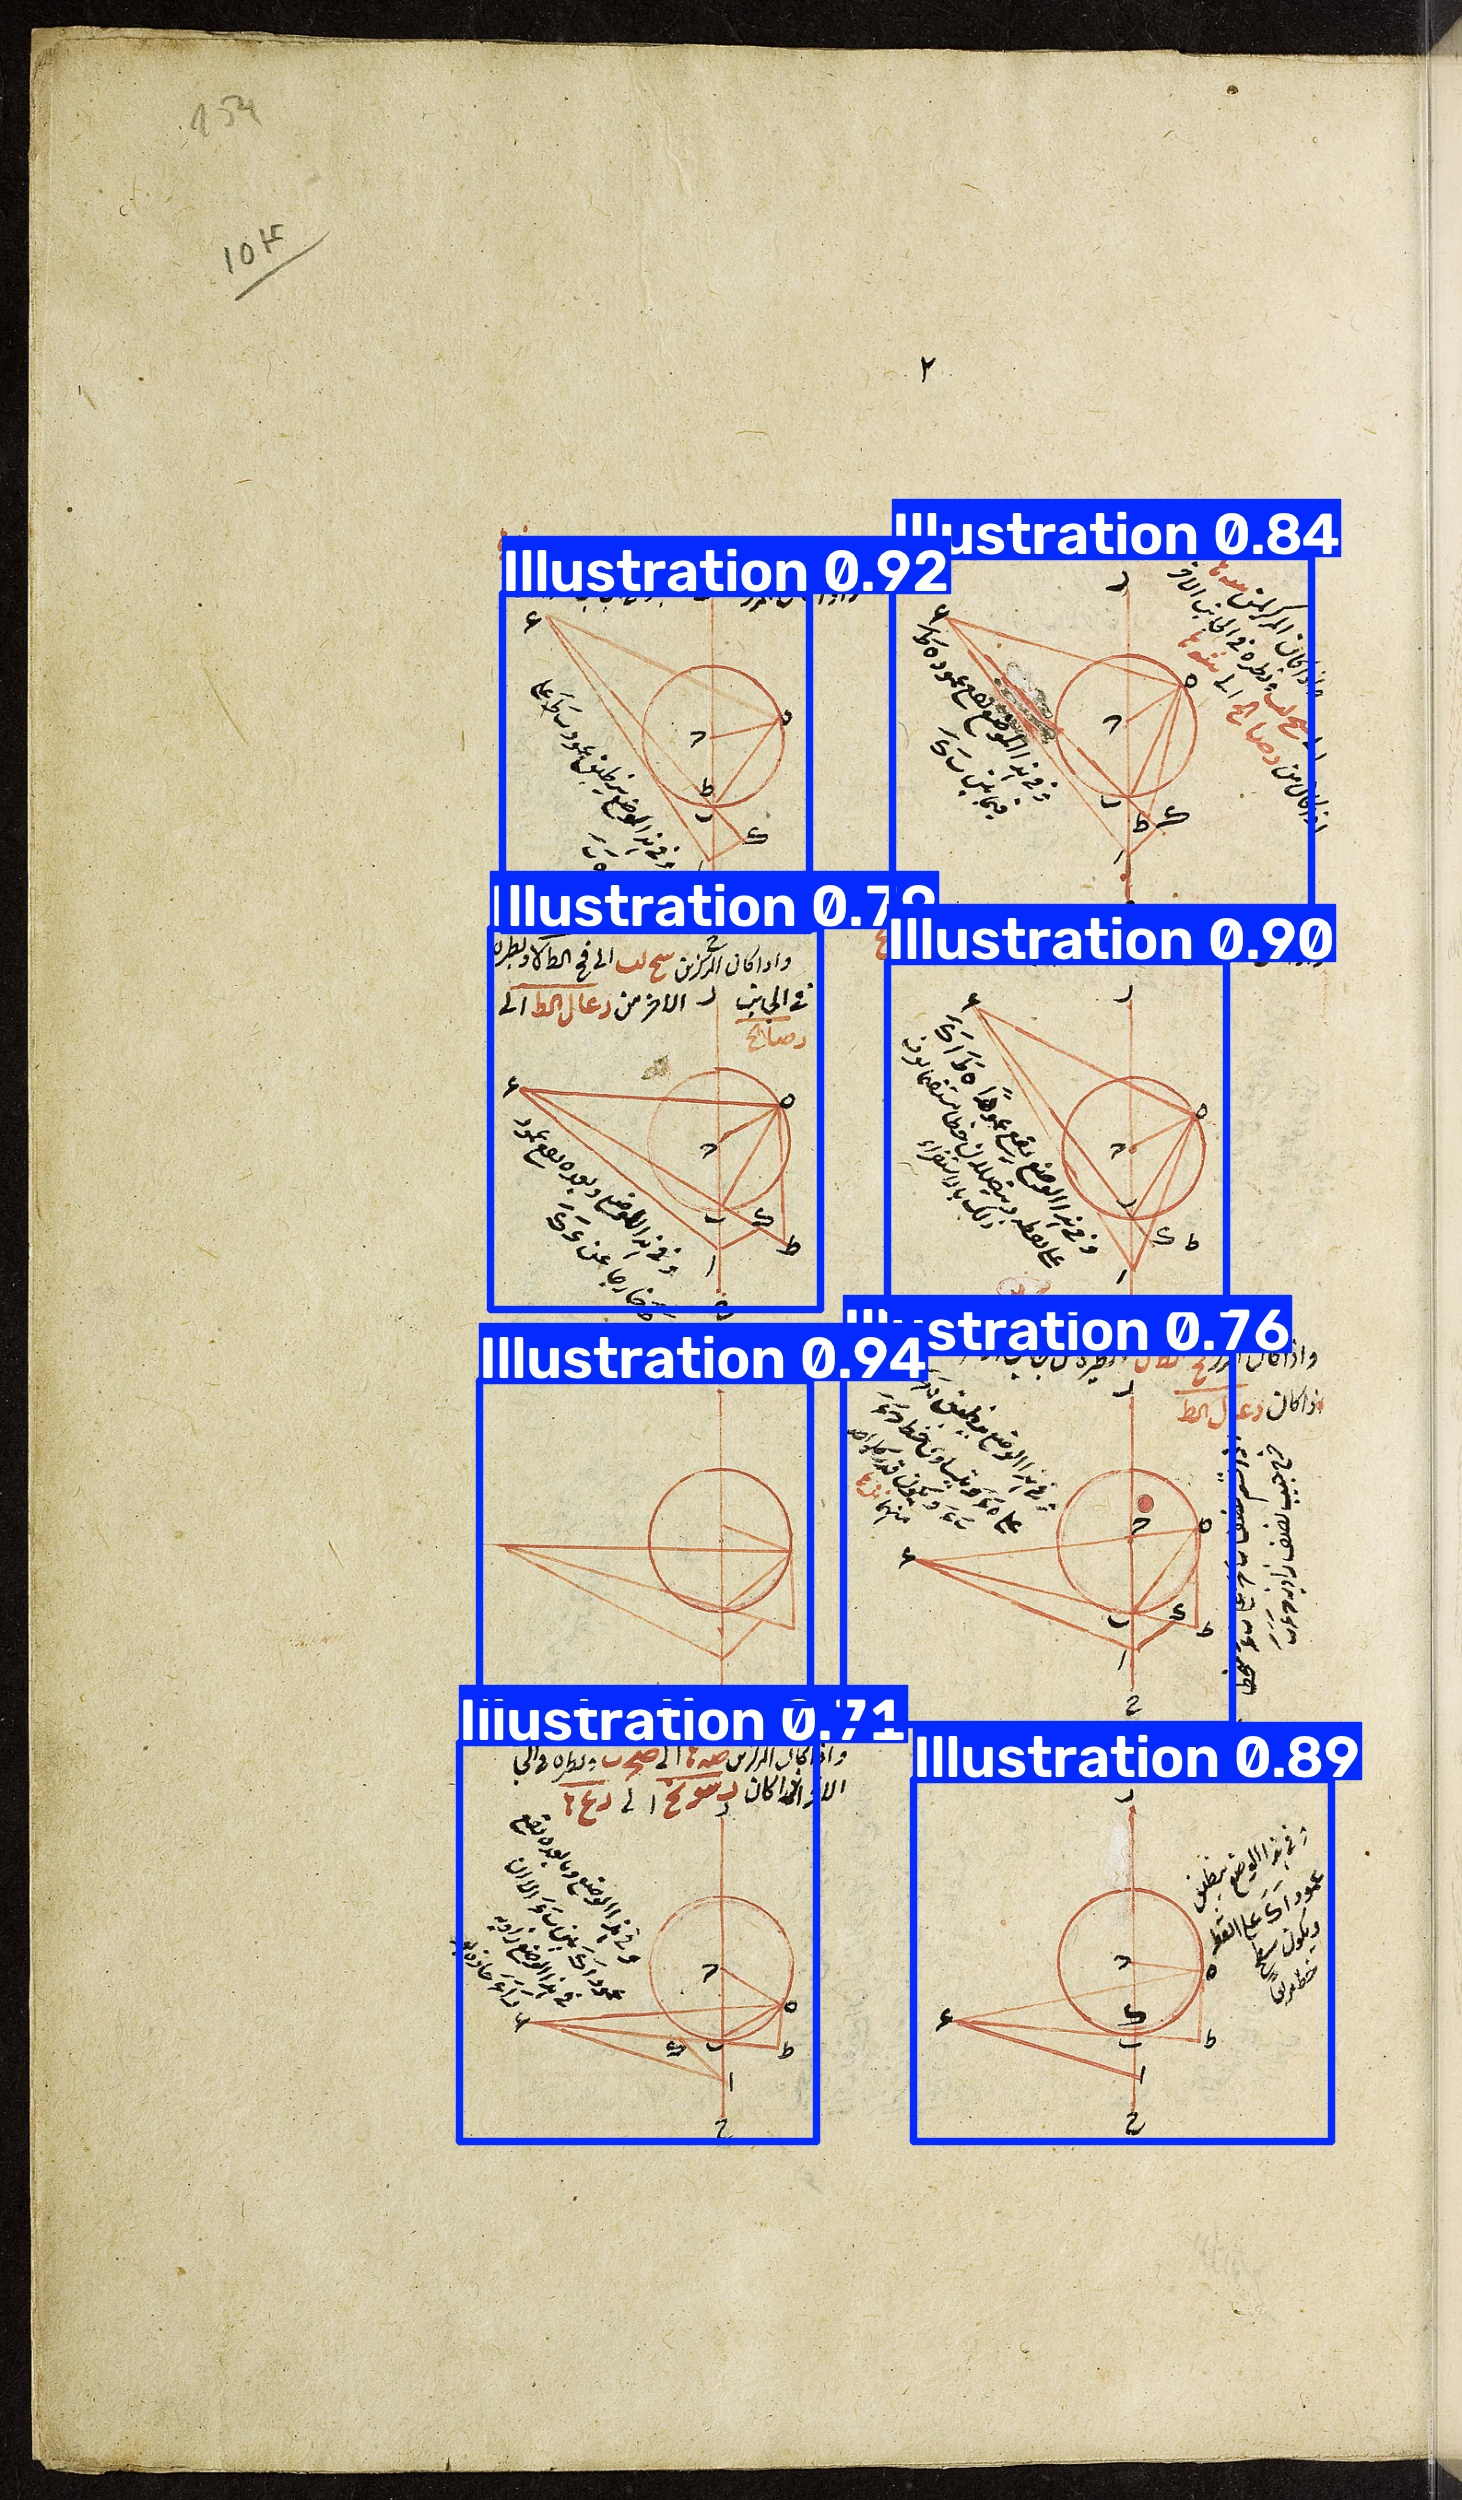
\includegraphics[scale=0.09]{img/detection.jpg}
            \caption{\textbf{Détection d'objets :} Exemple de détection produite par un modèle entraîné sur GenHisDoc. Ici le modèle détecte des illustrations sans hiérarchie ni organisation.}
            \label{fig:détection}
        \end{subfigure}
        \caption{Exemple de différence entre l'analyse de mise en page et la simple détection d'éléments dans la page.}
\end{figure}
    
\subsubsection{La segmentation au pixel :} Plus fine mais nettement plus coûteuses en annotation, la segmentation opère en attribuant une classe à chaque pixel de l'image comme montré dans la figure~\ref{fig:segexemple}. En vision patrimoniale, elle intervient principalement pour l'extraction de précision, qu'il s'agisse de tracer la ligne d'écriture exacte (\textit{baseline}) indispensable aux moteurs \gls{htr}, de détourer le fond d'un document dégradé ou d'isoler les contours complexes d'illustrations. La segmentation est l'une des pratiques les plus coûteuse, cependant c'est également un domaine très actif où des innovations comme \gls{sam}, un modèle rendu public par \textit{Meta} en 2023, permettent de transformer une détection en segmentation à un coût réduit\footnote{Alexander Kirillov, Eric Mintun, Nikhila Ravi, Hanzi Mao, Chloe Rolland, Laura Gustafson, Tete Xiao, Spencer Whitehead, Alexander C. Berg, Wan-Yen Lo, Piotr Dollár, Ross Girshick, \og Segment Anything \fg, publié sur ArXiv, URL : \href{https://arxiv.org/abs/2304.02643}{arXiv:2304.02643}}.

\subsection[Le triptyque Dataset / Modèle / Papier]{Le triptyque Dataset / Modèle / Papier, la compétition et les méthodes de mesure de performance biaisées qui en résultent.} 

Comme rappelé en introduction, le secteur de la vision artificielle appliquée aux documents s'est structuré autour d'un cycle de conférences avec des communications et compétitions internationales, à l'instar d'\gls{icdar} et d'\gls{icfhr}. Ces compétitions générales dépassent le seul cadre des applications aux corpus patrimoniaux et cela joue sur la manière dont le champ de recherche s'évalue et progresse. La publication d'un jeu de données donne alors lieu à l'entraînement d'un modèle de vision dont les performances seront validées par un article scientifique avec des métriques quantitatives. Cette focalisation sur la performance d'un modèle aide à choisir le meilleur outil pour réaliser une tâche de vision, mais n'est pas une bonne manière d'évaluer la scientificité d'un travail historique. L'acte méthodologique --- historiographique --- d'un projet de vision sur des documents patrimoniaux repose en réalité sur la construction de son ontologie d'annotation et la sur manière dont son jeu de données d'entraînement a été construit. 

% insérer une définition des métriques
\subsubsection{Les métriques de performances de base pour évaluer un modèle}

\begin{description}
    
        \item \textbf{Ground Truth (GT) / Vérité de terrain : }Le nombre total d'éléments d'intérêt (illustrations, schémas, etc.) réellement annotés à la main au sein du jeu de données de test. Il constitue la vérité de terrain de référence que le modèle cherche à retrouver.

        \item \textbf{Vrais Positifs (TP - \textit{True Positives}) :} Le nombre d'illustrations réelles correctement localisées et identifiées par le modèle.

        \item \textbf{Faux Positifs (FP - \textit{False Positives}) :} Le nombre d'erreurs par sur-détection. Il s'agit des cas où le modèle a prédit une illustration là où il n'y en avait pas (ex. une tache, un bloc de texte ou un élément d'ornementation non annoté).

        \item \textbf{Faux Négatifs (FN - \textit{False Negatives}) :} Le nombre d'omissions. Il représente les illustrations présentes dans les documents mais ignorées par le modèle.
    
\end{description}
    
\subsubsection{Les métriques de performance calculées pour évaluer un modèle:}

    \begin{description}
    
        \item \textbf{IoU Moyen (\textit{Intersection over Union}) :} L'indicateur de précision spatiale du tracé. L'IoU mesure le taux de recouvrement entre la boîte englobante prédite par le modèle ($B_p$) et la boîte réelle de la vérité de terrain ($B_{gt}$) :
        \begin{equation*}
            \text{IoU} = \frac{\text{Aire}(B_p \cap B_{gt})}{\text{Aire}(B_p \cup B_{gt})}
        \end{equation*}
        Plus l'IoU est élevé (ex. $> 0{,}85$), plus la localisation géométrique des boîtes englobantes est bonne. Cependant, l'IoU moyen mesure la qualité du tracé géométrique uniquement quand il y a un chevauchement entre une prédiction et une vérité terrain, et donc c'est une métrique masquant ainsi les faux négatifs (FN) et les faux positifs (FP). 

        \item \textbf{AP@50 / mAP@50 (\textit{La précision moyenne} (Average Precision) / \textit{mean Average Precision}) :} La métrique de référence en détection d'objets. Le seuil \texttt{@50} indique qu'une détection est considérée comme valide si son IoU avec la vérité de terrain est supérieur ou égal à $0{,}50$. L'AP calcule l'aire sous la courbe Précision/Rappel en balayant tous les seuils de confiance possibles (de $0$ à $1$), fournissant une évaluation globale de la capacité du modèle indépendamment d'un réglage particulier.
        
        l'AP porte sur une seule classe spécifique : C'est la Précision Moyenne calculée pour une seule catégorie d'objets.
        
        La mAP porte sur l'ensemble des classes détectées : Elle correspond à la moyenne des AP50 calculée sur l'ensemble des classes du jeu de données.

        \item \textbf{Précision :} La proportion de détections correctes parmi l'ensemble des prédictions effectuées par le modèle à un seuil de confiance donné :
        \begin{equation*}
            \text{Précision} = \frac{\text{Instances pertinentes récupérées (TP)}}{\text{Toutes les instances récupérées (TP + FP)}}
        \end{equation*}
        Dans le cadre de l'analyse automatique de documents, une précision élevée indique que presque tout ce que le modèle identifie comme étant un élément cible l'est réellement. Une précision élevée garantit à l'utilisateur que les boîtes générées contiennent très peu de faux bruit.

        \item \textbf{Rappel (\textit{Recall}) :} La proportion d'illustrations réellement retrouvées par le modèle par rapport au total des illustrations présentes dans le corpus :
        \begin{equation*}
            \text{Rappel} = \frac{\text{Instances pertinentes récupérées (TP)}}{\text{Toutes les instances pertinentes récupérées (TP + FN)}}
        \end{equation*}
        Pour une étude sérielle ou un inventaire, l'historien recherche l'exhaustivité. Il est souvent préférable d'avoir un modèle qui génère un peu de \og bruit \fg{} (Faux Positifs) que l'on éliminera rapidement à l'œil nu, plutôt qu'un modèle trop prudent qui omet des occurrences rares (Faux Négatifs). Un rappel élevé indique que le modèle ne rate presque aucune illustration dans un document.

        \item \textbf{Score F1 :} C'est la moyenne harmonique (moyenne entre des ratios, des taux ou des proportions) entre la Précision et le Rappel :
        \begin{equation*}
            \text{F1} = 2 \times \frac{\text{Précision} \times \text{Rappel}}{\text{Précision} + \text{Rappel}}
        \end{equation*}
        Il offre une mesure synthétique équilibrée du compromis entre exhaustivité (Rappel) et pertinence (Précision) à un seuil opérationnel fixe (ex. $\text{Conf} \ge 0{,}25$ ou $0{,}50$). Le Score F1 calculé à un seuil de confiance fixe est la métrique la plus pragmatique : elle indique l'équilibre réel entre exhaustivité et exactitude lors du déploiement du modèle sur un corpus de travail.
\end{description}

Dans le cadre des travaux menés sur le projet AIKON où nous travaillons sur la détection d'objets dans des documents, les trois métriques les plus pertinentes sont \textbf{le Rappel}, \textbf{la Précision} et \textbf{le Score F1}. Cependant pour d'autres tâches comme la segmentation de ligne d'écriture (\textit{Baseline Detection}), certaines métriques comme l'\textbf{Intersection over Union} à un seuil très discriminant (ex. $\text{Chevauchement} \ge 0{,}90$) deviennent primordiales pour éviter de mélanger les lignes d'écriture entre elles. Dans un projet visant à alimenter automatiquement une base de données iconographique, l'absence de bruit est privilégiée (pas de FP) et donc une précision élevée par rapport à son rappel ; inversement, lors d'une opération de dépouillement ou d'inventaire systématique des illustrations d'un manuscrit, le chercheur vise l'exhaustivité (absence de faux négatifs), ce qui exige un rappel élevé par rapport à la précision.

\section[De la prédiction à la connaissance]{De la prédiction géométrique à la connaissance historique : post-traitement, interprétation et structuration des résultats}

Dans le premier chapitre, nous avions vu que jusqu'aux alentours de 2010 s'affrontaient deux paradigmes. Le \textit{paradigme centré sur le modèle}, où l'amélioration technique amène à de meilleures performances, et le \textit{le paradigme centré sur la qualité des données}, où la qualité, la quantité et la diversité des données d'entraînement qui permettent de passer au-delà des impasses de l'approche centrée sur le modèle. Cependant, dans la partie précédente, nous avons conclu que pour une utilisation érudite comme en sciences historiques, la scientificité de l'utilisation de la vision artificielle passait d'abord par l'acte méthodologique de construction de l'ontologie d'annotation et de la manière dont les annotations sont conduites. En effet, le modèle n'apprend pas à \og voir \fg le document ou l'œuvre de manière neutre, il apprend à reproduire la grille de lecture définie par le schéma d'annotation sur de nouvelles images\footnote{Johannes Jakubik, Michael Vössing, Niklas Kühl, Jannis Walk, Gerhard Satzger, \og Data-Centric Artificial Intelligence \fg, publié sur ArXiv et accepté pour publication dans \textit{Business \& Information Systems Engineering}, pp.507–515, 2024, DOI: \href{https://arxiv.org/abs/2212.11854v4}{arXiv:2212.11854v4}}. À architecture égale, c'est la qualité des données qui produit la majorité des gains de performances et de possibilités d'utilisations. 

\subsection[La fabrique de la vérité de terrain]{La fabrique de la vérité de terrain (\textit{Ground Truth}) : L'importance de faire perdurer un écosystème de la vision patrimoniale}

Le but scientifique d'AIKON et de ses projets partenaires est d'étudier les méthodes d'interaction possibles entre un environnement technique et des spécialistes. Cela permet de produire de grands volumes de données de qualité de manière semi-automatique. Cependant, dans l'objectif de réutiliser ces données, de les mettre à disposition et de mettre en place un cercle vertueux d'amélioration continue de l'outil grâce aux résultats produits, il faut pouvoir superviser la grille de lecture qui lui est appliquée. Une bonne ontologie d'annotation permet à la fois de couper court à la majorité des ambiguïtés pour les annotateurs humains et de réduire le travail de correction en sortie de détection.

\subsubsection{Le découplage indispensable entre la structure physique et la  fonction sémantique}

La plupart des vocabulaires contrôlés utilisés comportent en moyenne cinq à six classes, avec un maximum autour d'une douzaine. L'une des erreurs méthodologiques majeures que l'on retrouve dans les jeux de données pour l'analyse de documents historiques consiste à mélanger la description visuelle et l'interprétation fonctionnelle. Dans la plupart des cas, les classes proposées sont mal adaptées aux documents historiques et, généralement, le vocabulaire utilisé ne sépare pas strictement l'analyse visuelle de la mise en page et la fonction textuelle ou sémantique. Nous notons également, dans la majorité des jeux de données historiques, l'absence des données tabulaires et des estampilles au sein des ontologies proposées.

Par exemple, le dataset S-VED\footnote{Jochen Büttner, Julius Martinetz, Hassan El-Hajj, Matteo Valleriani, \og CorDeep and the Sacrobosco Dataset: Detection of Visual Elements in Historical Documents \fg, dans \textit{Journal of Imaging}, pp.~285-303, 2022} propose une ontologie relativement simple constituée de quatre classes :
\begin{itemize}
	\item \textit{Illustration}
	\item \textit{Lettrine}
	\item \textit{Ornementation}
	\item \textit{Marque d'imprimeur}
\end{itemize}

\textit{Illustration}, \textit{Lettrine} et \textit{Ornementation} décrivent des éléments asémantiques (on ne fait pas de différence entre les types d'illustrations) et généraux (ces trois classes peuvent être utilisées sur des manuscrits comme sur des imprimés). Cependant, la classe \textit{Marque d'imprimeur} porte à la fois une information visuelle (une illustration) et sémantique (l'information véhiculée par l'illustration). De plus, les marques d'imprimeur constituent une spécificité propre aux livres imprimés, ce qui limite la réutilisation directe de l'ontologie du dataset S-VED ou exige un travail de correction sur les données. Attention, il est important de comprendre que le non-respect de ces règles ne rend pas un jeu de données inutile ou mauvais, mais il sera forcément plus difficile de le traiter et de le croiser avec d'autres jeux de données s'il ne se conforme pas à ces principes.

\begin{figure}[htbp]
	\centering
	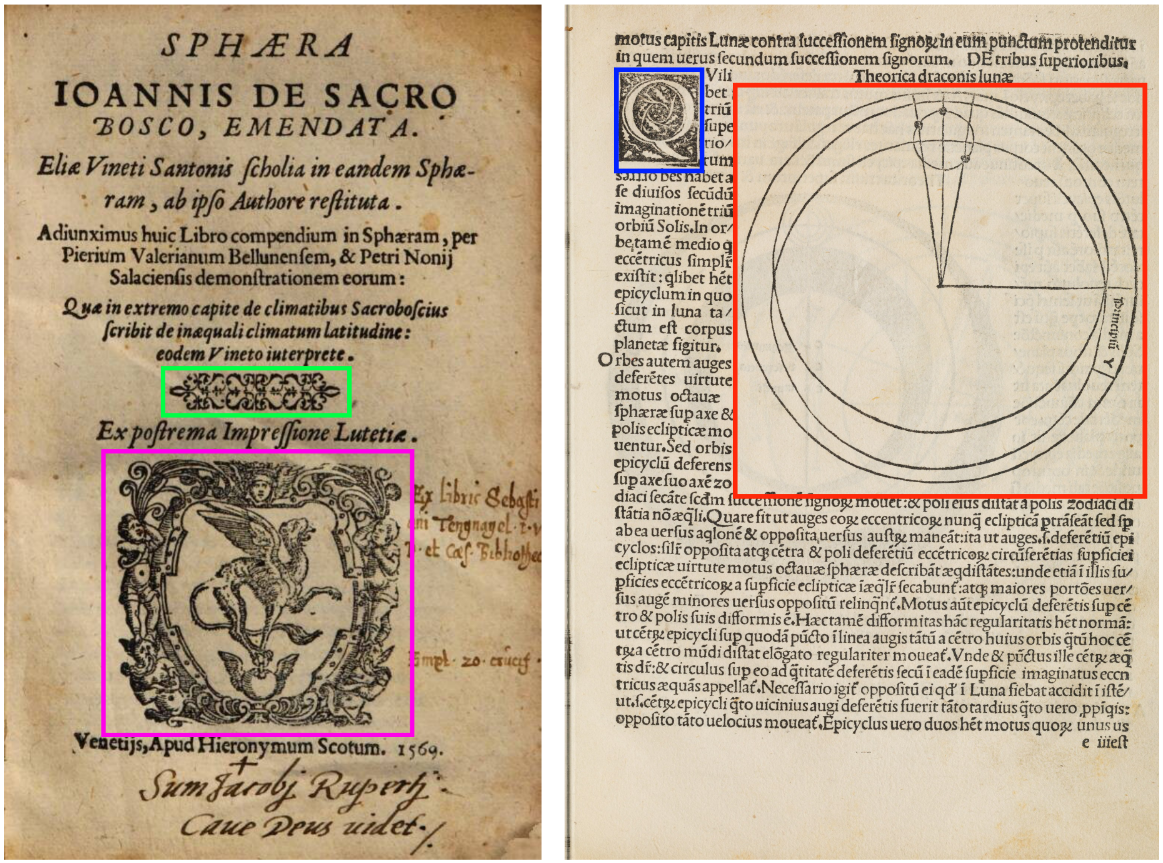
\includegraphics[scale=0.3]{img/s-ved.png}
	\caption{Deux pages du dataset S-VED (2022) représentant les quatre classes du vocabulaire de description du document.}
	\label{fig:s-ved}
\end{figure}

Pour notre tâche de constitution de corpus, nous avons donc dû réaligner de nombreux jeux de données présentant ce genre de défauts dans leurs vocabulaires contrôlés, qu'il s'agisse de descriptions de manuscrits ou d'imprimés. De plus, nous étions soumis à des contraintes de temps (l'ontologie ne devait pas être trop complexe) et de ressources humaines (un travail confié à un profil généraliste confronté à une grande diversité de typologies documentaires). Nous avons donc obéi à une règle en trois points : les classes au sein de notre ontologie doivent être uniquement visuelles (asémantiques), applicables à plusieurs typologies de documents comme les manuscrits et les imprimés (généralistes), et elles ne doivent pas pouvoir se confondre (absence de chevauchements ou \textit{overlaps}). Nous avons nommé cette règle \gls{agc}.

\begin{table}
\centering
\ra{1.25}
\caption{Comparaison des ontologies utilisées selon notre principe \gls{agc} dans l'annotation de différents jeux de données}
\label{tab:datasets-comparison}
	\begin{tabular}{lcccc}
	\toprule
	\textbf{Nom} & \textbf{Asemantic} & \textbf{Generalistic} & \textbf{Classes overlaps} & \textbf{Format} \\
	\midrule
	IlluHisDoc & {\color{red}\faClose} & {\color{green}\faCheck} & {\color{red}\faClose} & Per pixel  \\
	S-VED & {\color{red}\faClose} & {\color{green}\faCheck} & {\color{red}\faClose} & Per pixel  \\
	Horae-LSv2 & {\color{red}\faClose} & {\color{red}\faClose} & {\color{red}\faClose} & Yolo  \\
	SegmOnto & {\color{green}\faCheck} & {\color{green}\faCheck} & {\color{red}\faClose} & other XML \\
	Newspaper Datasets & {\color{red}\faClose} & {\color{red}\faClose} & {\color{red}\faClose} & \dots \\
	PrimA & {\color{green}\faCheck} & {\color{red}\faClose} & {\color{red}\faClose} & other XML \\
	DIVAHisDB & {\color{green}\faCheck} & {\color{red}\faClose} & {\color{red}\faClose} & PAGE XML \\
	DMAS2019 & {\color{red}\faClose} & {\color{red}\faClose} & {\color{red}\faClose} & PAGE XML \\
	\textbf{GenHisDoc} & {\color{green}\faCheck} & {\color{green}\faCheck} & {\color{green}\faCheck} & Yolo \\
\bottomrule
\end{tabular}
\end{table}

\subsubsection{La réalité humaine de la tâche d'annotation}

Durant la création d'une ontologie, le chercheur ou la chercheuse va tendre vers une forme d'exhaustivité descriptive pour rendre compte de la complexité de ses sources. Or, la vision par ordinateur fait face à des contraintes statistiques strictes qui entrent en contradiction directe avec ce besoin de précision historiographique. 

Cette volonté d'exhaustivité se heurte à ce que l'on nomme \textit{long-tail distribution}\footnote{Chongsheng Zhang, George Almpanidis, Gaojuan Fan, Binquan Deng, Yanbo Zhang, \og A Systematic Review on Long-Tailed Learning \fg, publié sur ArXiv, DOI : \href{https://doi.org/10.48550/arXiv.2408.00483}{https:\/\/doi.org/10.48550\/arXiv.2408.00483}} des classes au sein des annotations du dataset. Concevoir une ontologie dotée de dizaines de catégories très spécifiques (les annotations de lettrines au sein de Horae, par exemple) crée un déséquilibre statistique. Le modèle manquera d'exemples d'entraînement pour les classes les plus rares, ce qui se traduira par un taux de rappel quasi nul pour ces dernières. De plus, cette grande variété dans les choix d'annotation démultiplie la complexité de la tâche d'annotation humaine. Ce travail, exigeant et répétitif, repose très souvent sur des opérateurs humains (étudiants, stagiaires, vacataires) soumis à une forte charge cognitive. Plus le nombre de classes augmente, plus l'ambiguïté grandit face à un document historique souvent dégradé, ce qui fait inévitablement chuter l'accord inter-annotateurs (\gls{iaa}) et produit ainsi un jeu de données bruité. 

Pour pallier ce problème tout en préservant les fonctionnalités nécessaires à la recherche, Il existe deux solutions : 

Pour AIKON, au vu des moyens et du temps disponible, nous avons décidé d'utiliser une ontologie minimale avec des classes très englobantes. Par exemple, \textit{Illustration} englobe toutes les illustrations d'un livre d'heures, mais également les schémas mathématiques d'un manuscrit ou les photographies d'une page de journal. Cela diminue forcément la précision d'un modèle, mais c'est le choix que nous avons fait pour GenHisDoc. 

Une autre solution réside dans la construction d'une ontologie hiérarchique\footnote{Ghassan Beydoun, Antonio A. Lopez-Lorca, Francisco García-Sánchez, Rodrigo Martínez-Béjar, \og How do we measure and improve the quality of a hierarchical ontology? \fg, dans \textit{Journal of Systems and Software}, n°84, vol 12, pp. 2363-2373, 2011}. Il s'agit d'un vocabulaire contrôlé qui utilise des relations de subsomption (le principe du \textit{is-a} ou \og est un \fg). Cette structuration en arbre permet de regrouper les classes rares sous des macro-catégories plus larges. D'un point de vue informatique, cela autorise l'entraînement du modèle avec une fonction de perte hiérarchique (\textit{hierarchical loss}). Ainsi, si le réseau de neurones, ou l'annotateur humain en amont, hésite sur la sous-classe exacte d'un objet en raison d'une ambiguïté visuelle, il peut au moins assigner ou prédire correctement la classe supérieure (par exemple, identifier formellement une \textit{Lettrine} plutôt que de se tromper entre une lettrine historiée et une lettrine enluminée). L'erreur est alors atténuée et l'accord inter-annotateur beaucoup plus fort, le modèle n'est donc pas brutalement pénalisé pour une classification imparfaite au niveau de la sous-classe, et la tâche de l'annotateur est potentiellement allégée.

% parler du fait que corriger est en fait plus long qu'annoté une page vierge

\subsection{Vers une \og nouvelle économie de l'érudition \fg{} : la vision et les pratiques des chercheurs}

La création d'une vérité de terrain en vision par ordinateur est, nous l'avons vu, une tâche chronophage et coûteuse, tant dans la modélisation conceptuelle (l'ontologie) du document que dans la production effective des annotations. Pour répondre à ces contraintes de temps et de moyens, le champ de la vision artificielle appliquée aux documents historiques s'oriente vers le développement de projets et de plateformes de partage de jeux de données, conçus pour favoriser leur réutilisation et leur interopérabilité.

\subsubsection{Du « goût de l'archive » à une recherche collective : les enjeux méthodologiques de l'intermédiation numérique}

L'histoire est une discipline profondément auto-réflexive, traditionnellement attachée au contact direct, physique et sensuel avec la source. Ce que l'historienne Arlette Farge a nommé le \og goût de l'archive \fg\footnote{Arlette Farge, \textit{Le Goût de l'archive}, éditions du Seuil, 1989.} repose sur une relation intime entre le chercheur individuel et le document matériel. Or, l'introduction de la vision artificielle dans le travail de dépouillement modifie cette relation en imposant une intermédiation technologique qui peut sembler opaque. 

Les historiens se sont saisis de l'outil informatique avec deux utilisations principales : l'édition de sources et la mise en base de données qui permettent de partager des résultats. Dans le domaine de la vision, il existe déjà des outils et des modèles capables de produire des résultats utiles, mais la barrière d'entrée lié à la complexité de réutilisation des données et des moyens à investir pour pouvoir produire de nouvelles données sont trop élevée pour la plupart des chercheurs menant des travaux individuels ou pour la plupart des laboratoires universitaires en général. Quand on veut y intégrer des méthodes de \textit{machine learning}, la recherche ne peut plus s'envisager comme une démarche purement solitaire. Elle devient dépendante d'infrastructures techniques complexes (serveurs de calcul) et d'un travail collectif en amont (ingénieurs, annotateurs, hébergement).

En France, l'initiative la plus proche d'une telle infrastructure est le projet Gallicorpora. Conçu pour la constitution de jeux de données d'entraînement et le développement d'outils de conversion des standards de la \gls{bnf} vers la \gls{tei}, cet écosystème fournit des corpus d'images finement annotées combinant transcription textuelle et segmentation de la mise en page pour des imprimés allant du XVe au XIXe siècle. Un autre exemple sont les jeux de données de l'équipe \gls{almanach} de l'\gls{inria} avec les jeux de données CATmus\footnote{Thibault Clérice, Ariane Pinche, Malamatenia Vlachou-Efstathiou, Alix Chagué, Jean-Baptiste Camps, et al.. \og CATMuS Medieval: A multilingual large-scale cross-century dataset in Latin script for handwritten text recognition and beyond. \fg communication pour \textit{2024 International Conference on Document Analysis and Recognition (ICDAR)}, pp.174-194, 2024} puis CoMMA\footnote{Thibault Clérice, Simon Gabay, Malamatenia Vlachou-Efstathiou, Ariane Pinche, Benoît Sagot. \og CoMMA, a Large-scale Corpus of Multilingual Medieval Archives \fg, publié sur HAL, 2025,  Hal ID : hal-05299220v1⟩}. Toutefois, pour les autres tâches de vision par ordinateur, comme l'analyse de mise en page avancée, la segmentation ou la détection d'éléments visuels, il n'existe toujours pas d'initiative fédératrice assurant la mutualisation des données produites. De plus, à l'exception notable de la démarche SegmOnto, la communauté manque encore de benchmarks permettant d'évaluer l'efficacité des ontologies et d'attester que les données générées répondent à un véritable intérêt scientifique.

Dès lors, comment définir ce qui constitue une \og bonne \fg{} ontologie pour l'étude des documents historiques, et sur quels critères la privilégier face à une autre ? Comme nous l'avons vu, son évaluation ne saurait se limiter aux seules métriques de performances algorithmique. Pour un usage historique, une ontologie pertinente se juge donc en deux temps : opératoire et heuristique.

D'un côté, elle doit assurer une robustesse statistique en limitant l'ambiguïté pour les annotateurs humains et la machine, un défi auquel tentent de répondre des principes de conception que nous avons évoqué plus tôt. De l'autre, sa valeur réelle se mesure à son intêret scientifique. Face à deux vocabulaires contrôlés concurrents, l'ontologie supérieure est celle qui garantit la meilleure interopérabilité des données produites, permettant ainsi le croisement de corpus matériels hétérogènes.

Pour le choix entre deux vocabulaires contrôlés concurrent, l'ontologie supérieure est en réalité celle qui garantit la meilleure interopérabilité des données produites. Nous laissons donc derrière nous une partie des jeux de données ayant des systèmes d'annotations exhaustives souvent confinés à des projets uniques, au profit de grilles de lecture articulées autour du principe de généralisation. 

\subsubsection{Le standard \gls{iiif} et ses atouts pour l'Open Data}

En informatique, la validité d'une démarche repose sur la reproductibilité des résultats, et donc la possibilité de réexécuter un traitement sur un même jeu de données. En histoire, la scientificité d'une démonstration s'appuie sur la critique des sources et la possibilité, pour les pairs, de vérifier l'appareil critique. La rencontre entre ces deux exigences démontre que la scientificité de l'utilisation de méthodes de machine learning pour l'analyse de documents passe par l'ouverture des données d'entrainement.

Dans ce contexte, l'adoption de standards techniques partagés devient incontournable, au premier rang desquels figure le protocole \gls{iiif}. Ce cadre a profondément transformé l'accès aux corpus patrimoniaux en permettant de manipuler, de comparer et d'annoter des images à très haute résolution provenant de différentes institutions (\gls{bnf}, bibliothèques universitaires, musées) sans forcément avoir à télécharger, ni à dupliquer ces lourds fichiers. Plus encore, grâce aux standards du Web sémantique (comme le \textit{Web Annotation Data Model}), les prédictions générées par la vision artificielle (boîtes englobantes, polygones de segmentation) peuvent être partagées sous forme de surcouches textuelles légères (fichiers JSON) pointant directement vers les \gls{uri} des images distantes. L'utilisation de \gls{iiif} au sein d'application de vision permet un meilleur usage et partage des données des institutions patrimoniales et des données de la recherche qui en découlent. 

L'intégration native de \gls{iiif} au sein du projet AIKON s'inscrit pleinement dans cette dynamique. En proposant un environnement utilisateur capable de se brancher directement sur les entrepôts numériques des institutions patrimoniales, l'application facilite la constitution de corpus personnalisés et le déploiement de modèles de détection sans friction technique. Ce choix architectural contribue à une meilleure diffusion des données de la recherche : les chercheurs peuvent importer leurs sources, exécuter une tâche de détection, puis exporter et partager leurs résultats sous des formats ouverts. Cet écosystème interopérable est ainsi pensé pour s'insérer naturellement dans le cycle de vie de la donnée patrimoniale et encourager un partage continu des connaissances au sein de la communauté scientifique.